% \documentclass[handout]{beamer}
\documentclass[aspectratio=1610]{beamer}

\mode<presentation>
{
  % \usefonttheme[onlymath]{serif}
  \usetheme{default}
  % \usetheme{Warsaw}
  % \usetheme{Malmoe}
  % \useinnertheme{circles}
  % \useoutertheme{default}
  % \useinnertheme{rounded}

  \setbeamercovered{transparent=1}
}

\usepackage[english]{babel}
\usepackage[latin1]{inputenc}
\usepackage{alltt,listings,multirow,ulem,siunitx}
\usepackage[absolute,overlay]{textpos}
\TPGrid{1}{1}
\usepackage{pdfpages}
\usepackage{animate}
\usepackage{ulem}
\usepackage{multimedia}
\usepackage{multicol}
\newcommand\hmmax{0}
\newcommand\bmmax{0}
\usepackage{bm}
\usepackage{comment}
\usepackage{subcaption}
\usepackage{amscd}
\usepackage{xspace}

\NewDocumentCommand{\rot}{O{45} O{1em} m}{\makebox[#2][l]{\rotatebox{#1}{#3}}}

% font definitions, try \usepackage{ae} instead of the following
% three lines if you don't like this look
\usepackage{mathptmx}
\usepackage[scaled=.90]{helvet}
% \usepackage{courier}
\usepackage[T1]{fontenc}
\usepackage{tikz}
\usetikzlibrary{decorations.pathreplacing}
\usetikzlibrary{shadows,arrows,shapes.misc,shapes.arrows,shapes.multipart,arrows,decorations.pathmorphing,backgrounds,positioning,fit,petri,calc,shadows,chains,matrix,mindmap}

\newcommand\vvec{\bm v}
\newcommand\bvec{\bm b}
\newcommand\bxk{\bvec_0 \times \kappa_0 \cdot \nabla}
\newcommand\delp{\nabla_\perp}

% \usepackage{pgfpages}
% \pgfpagesuselayout{4 on 1}[a4paper,landscape,border shrink=5mm]

\usepackage{JedMacros}
\usepackage{standalone}

\newcommand{\timeR}{t_{\mathrm{R}}}
\newcommand{\timeW}{t_{\mathrm{W}}}
\newcommand{\mglevel}{\ensuremath{\ell}}
\newcommand{\mglevelcp}{\ensuremath{\mglevel_{\mathrm{cp}}}}
\newcommand{\mglevelcoarse}{\ensuremath{\mglevel_{\mathrm{coarse}}}}
\newcommand{\mglevelfine}{\ensuremath{\mglevel_{\mathrm{fine}}}}

%solution and residual
\newcommand{\vx}{\ensuremath{x}}
\newcommand{\vc}{\ensuremath{\hat{x}}}
\newcommand{\vr}{\ensuremath{r}}
\newcommand{\vb}{\ensuremath{b}}

%operators
\newcommand{\vA}{\ensuremath{A}}
\newcommand{\vP}{\ensuremath{I_H^h}}
\newcommand{\vS}{\ensuremath{S}}
\newcommand{\vR}{\ensuremath{I_h^H}}
\newcommand{\vI}{\ensuremath{\hat I_h^H}}
\newcommand{\vV}{\ensuremath{\mathbf{V}}}
\newcommand{\vF}{\ensuremath{F}}
\newcommand{\vtau}{\ensuremath{\mathbf{\tau}}}


\title{Library Interface Design and Performance Portability}

%Library developers seek to effectively serve the needs of present and future users while providing extension points for new developers to start contributing and quickly realize their impact.  This involves providing powerful abstractions that are not too abstract to reason about, often decomposing familiar algorithms into constituent parts that can be recomposed to create new algorithms or variants with little or no software development effort, and providing diagnostics and debugging tools.  When striving for performance, library developers must pay attention to interface granularity to enable vectorization, various forms of blocking for locality, and fusion.  The flavor of a library is often defined by its choice of programming technology, from traditional fixed-ABI to template metaprogramming to just-in-time (JIT) compilation.  We provide examples of interface tradeoffs by way of libCEED, a new performance portable algebraic discretization library that provides optimized finite element/spectral element infrastructure to a range of applications.
\author{{\bf Jed Brown}, Jeremy Thompson, Valeria Barra}

% - Use the \inst command only if there are several affiliations.
% - Keep it simple, no one is interested in your street address.
% \institute
% {
%   Mathematics and Computer Science Division \\ Argonne National Laboratory
% }

\date{SIAM CSE, Spokane, 2019-02-25 \\[1em]
This talk: \url{https://jedbrown.org/files/20190225-PerfPortability.pdf}}

% This is only inserted into the PDF information catalog. Can be left
% out.
\subject{Talks}


% If you have a file called "university-logo-filename.xxx", where xxx
% is a graphic format that can be processed by latex or pdflatex,
% resp., then you can add a logo as follows:

% \pgfdeclareimage[height=0.5cm]{university-logo}{university-logo-filename}
% \logo{\pgfuseimage{university-logo}}



% Delete this, if you do not want the table of contents to pop up at
% the beginning of each subsection:
% \AtBeginSubsection[]
% {
% \begin{frame}<beamer>
%   \frametitle{Outline}
%   \tableofcontents[currentsection,currentsubsection]
% \end{frame}
% }

% \AtBeginSection[]
% {
%   \begin{frame}<beamer>
%     \frametitle{Outline}
%     \tableofcontents[currentsection]
%   \end{frame}
% }

% If you wish to uncover everything in a step-wise fashion, uncomment
% the following command:

% \beamerdefaultoverlayspecification{<+->}

\begin{document}
\lstset{language=C}
\normalem

\begin{frame}
  \titlepage
\end{frame}

\begin{frame}{What is performance portability?}
  \begin{itemize}
  \item Performs well across range of architectures and problem configurations with modest development and maintenance effort.
  \item All architectures require massive parallelism
    \begin{itemize}
    \item 28-core Xeon: dual-issue FMA with 16-lane registers, 6-cycle latency: 5376 in-flight flops
    \item About 4x more for V100
    \end{itemize}
  \item Architectural differences
    \begin{itemize}
    \item Persistent cache on CPU, big register space on GPU
    \item Programming model expression of coalesced loads (e.g., CUDA vs OpenMP/OpenACC)
    \item Tolerance for lane divergence (SIMT versus masked SIMD); what does compiler need to know/use?
    \end{itemize}
  \item Problem configurations: time to solution requirements (problem sizes)
    \begin{itemize}
    \item constitutive models, etc.
    \end{itemize}
  \end{itemize}
\end{frame}

\begin{frame}{HPGMG-FE on Edison, SuperMUC, Titan}
  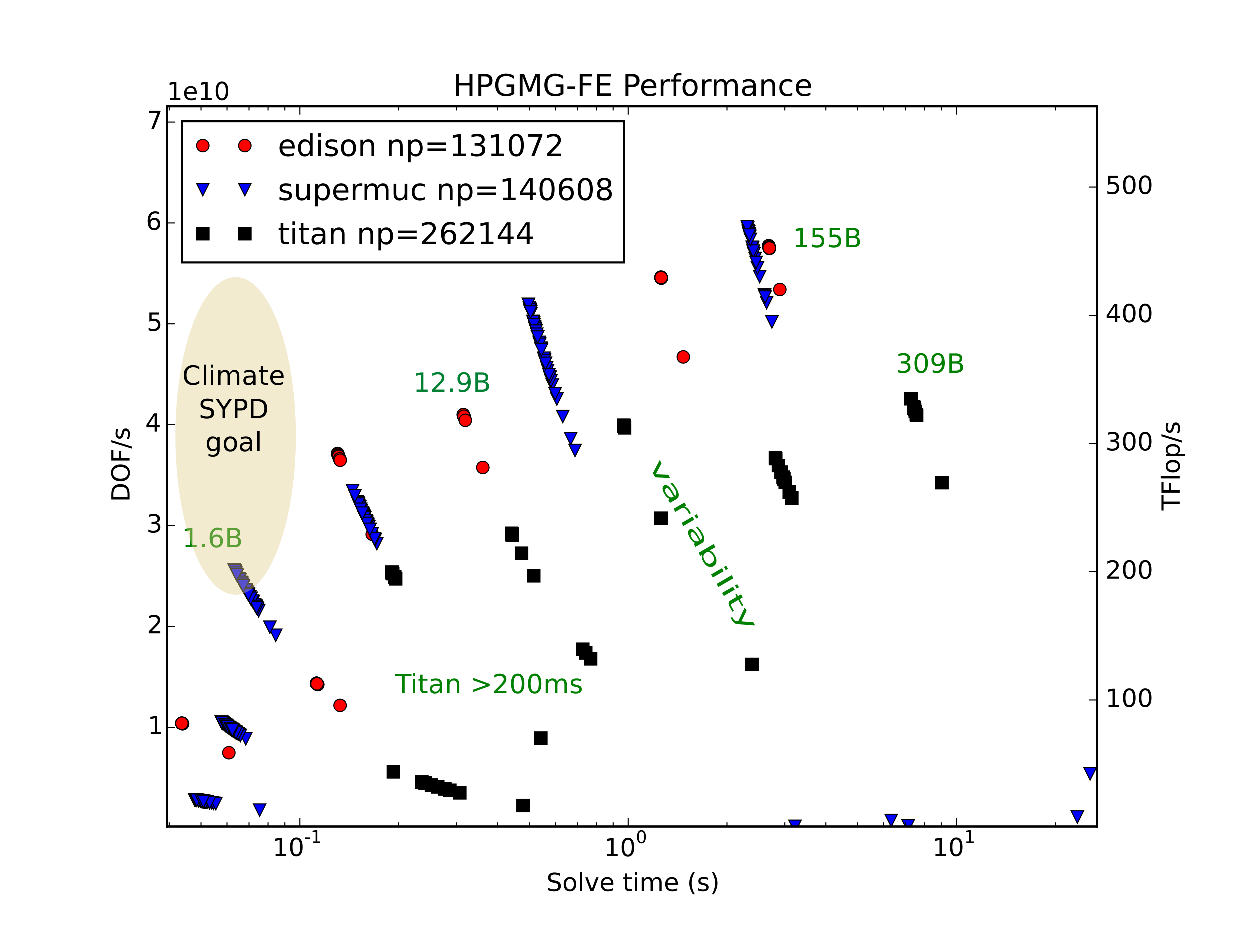
\includegraphics[width=.8\textwidth]{figures/hpgmg/range-edison-supermuc-titan-ann2.eps}
\end{frame}

\begin{frame}{Modest development and maintenance effort}
  \begin{itemize}
  \item Some custom code may be needed; how to leverage?
  \item Granularity of extensibility
    \begin{itemize}
    \item BLAS/LAPACK: Users compose large dense linear algebraic operations
    \item BLIS: Users implement packing schemes; reuse ``microkernel''
    \item Users implement different PDE, discretization, and constitutive models
    \item FEniCS: domain-specific language for finite element
    \end{itemize}
  \item Maintenance
    \begin{itemize}
    \item Interface stability for the extensible parts
    \item Ability to rapidly affect ``infrastructure'' (turtles all the way down?)
    \end{itemize}
  \end{itemize}
\end{frame}

\begin{frame}{Approaches}
  \begin{tabular}{lccccc}
    Type of software & \rot{Expressive} & \rot{Interoperable/Environment} & \rot{Contributors} & \rot{New architecture} & \rot{Packaging/Distribution} \\
    \midrule
    Library (LAPACK, FFTW, BLIS @MS129 $\downarrow$) & $-$ & $+$ & $+$ & 0 & $+$ \\
    Dynamic/extensible Library (libCEED) & 0 & $+$ & $+$ & plugin & if stable ABI \\
    Template Library (Kokkos @MS129) & 0 & 0 & 0 & $+$ & recompile \\
    DSL/code generation/JIT (Firedrake) & $+$ & $-$ & 0 & $+$ & ? \\
    New Language (Chapel) & $+$ & $-$ & $-$ & ? & ? \\
    \bottomrule
  \end{tabular}
\end{frame}

\begin{frame}
  \includegraphics[width=\textwidth]{figures/karlrupp/flop-per-byte-dp.pdf} \\
  {\scriptsize [c/o Karl Rupp]}
\end{frame}

\begin{frame}[shrink=5]{Performance of assembled versus unassembled}
  \vspace{1ex}
  \includegraphics[width=\textwidth]{figures/TensorVsAssembly} \\
  \begin{itemize}
  \item Arithmetic intensity for $\Qk p$ elements
    \begin{itemize}
    \item $< \frac 1 4$ (assembled), $\approx 10$ (unassembled), $\approx 5$ to $10$ (hardware)
    \end{itemize}
  \item store Jacobian information at Gauss quadrature points, can use AD
  \end{itemize}
\end{frame}

\begin{frame}{libCEED: Code for Efficient Extensible Discretization}
  \begin{itemize}
  \item BSD-2 license, C library with Fortran interface
  \item Releases: v0.1 --- v0.3 (2018); v0.4 to be released in March
  \item Purely algebraic interface
  \item Extensible backends
    \begin{itemize}
    \item CPU: reference, blocked/vectorized, libXSMM
    \item OCCA (just-in-time compilation): CPU, OpenMP, OpenCL, CUDA
    \item MAGMA
    \item CUDA using NVRTC (Steven Roberts \& Yohann Dudouit, to be merged soon)
    \end{itemize}
  \item Platform for collaboration with vendors
  \item Minimal assumptions about execution environment, parallel decomposition
  \item Primary target: high order finite element methods
    \begin{itemize}
    \item $H^1, H(\mathrm{div}), H(\mathrm{curl})$
    \item Also of interest to spectral difference, etc.
    \item Exploit tensor product structure when possible
    \end{itemize}
  \end{itemize}
\end{frame}

\begin{frame}
  \includegraphics[width=\textwidth]{figures/ceed/libCEED-2.pdf}
\end{frame}

\begin{frame}{Quadrature Function}
  \begin{gather*}
    v^T F(u) \sim \int_\Omega v \cdot f_0(u, \nabla u) + \nabla v \tcolon f_1(u, \nabla u) \qquad
    v^T J w \sim \int_\Omega \begin{bmatrix} v \\ \nabla v \end{bmatrix}^T \begin{bmatrix} f_{0,0} & f_{0,1} \\ f_{1,0} & f_{1,1} \end{bmatrix} \begin{bmatrix} w \\ \nabla w \end{bmatrix} \\
    u = B_I \mathcal E_e u_L \qquad \nabla u = \frac{\partial X}{\partial x} B_{\nabla} \mathcal E_e u_L \\
    J w = \sum_e \mathcal E_e^T \begin{bmatrix} B_I \\ B_{\nabla} \end{bmatrix}^T
    \underbrace{\begin{bmatrix} I & \\ & \left( \frac{\partial X}{\partial x}\right)^T \end{bmatrix} W_q \begin{bmatrix} f_{0,0} & f_{0,1} \\ f_{1,0} & f_{1,1} \end{bmatrix} \begin{bmatrix} I & \\ & \left( \frac{\partial X}{\partial x}\right) \end{bmatrix}}_{\text{coefficients at quadrature points}} \begin{bmatrix} B_I \\ B_{\nabla} \end{bmatrix} \mathcal E_e w_L
  \end{gather*}
  \begin{itemize}
  \item $B$ and $B_\nabla$ are tensor contractions -- independent of element geometry
  \item Choice of how to order and represent gathers $\mathcal E$ and scatters $\mathcal E^T$
  \item Who computes the metric terms and other coefficients?
  \item Similar for Neumann/Robin and nonlinear boundary conditions
  \end{itemize}
\end{frame}

\begin{frame}[fragile]{Quadrature Functions}
  \begin{itemize}
  \item Multiple inputs and outputs
  \item Independent operations at each of \texttt{Q} quadrature points
    \begin{itemize}
    \item Ordering and number of elements not specified
    \end{itemize}
  \end{itemize}
  \begin{minipage}{0.5\textwidth}
    \begin{minted}{C}
      int L2residual(void *ctx, CeedInt Q,
                     const CeedScalar *const in[],
                     CeedScalar *const out[]) {
        const CeedScalar *u = in[0], *rho = in[1], *target = in[2];
        CeedScalar *v = out[0];
        #pragma omp simd
        for (CeedInt i=0; i<Q; i++)
          v[i] = rho[i] * (u[i] - target[i]);
        return 0;
      }
      CeedQFunctionAddInput(qf, "u", 1, CEED_EVAL_INTERP);
      CeedQFunctionAddInput(qf, "rho", 1, CEED_EVAL_INTERP);
      CeedQFunctionAddInput(qf, "target", 1, CEED_EVAL_INTERP);
      CeedQFunctionAddOutput(qf, "v", 1, CEED_EVAL_INTERP);
    \end{minted}
  \end{minipage}
\end{frame}

\begin{frame}{Building Operators}
  \begin{gather*}
    v^T F(u) \sim \int_\Omega v \cdot f_0(u, \nabla u) + \nabla v 
    \tcolon f_1(u, \nabla u) \\
    u = B_I \mathcal E_e u_L \quad \nabla u = \frac{\partial X}{\partial x} B_{\nabla} \mathcal E_e u_L
  \end{gather*}
  % \begin{gather*} v^T J w = \sum_e \mathcal E_e^T \begin{bmatrix} B \\ D \end{bmatrix}^T
  %   \underbrace{\begin{bmatrix} I & \\ & \left( \frac{\partial X}{\partial x}\right)^T \end{bmatrix} W_q \begin{bmatrix} f_{0,0} & f_{0,1} \\ f_{1,0} & f_{1,1} \end{bmatrix} \begin{bmatrix} I & \\ & \left( \frac{\partial X}{\partial x}\right) \end{bmatrix}}_{\text{coefficients at quadrature points}} \begin{bmatrix} B \\ D \end{bmatrix} \mathcal E_e w
  % \end{gather*}
  \begin{itemize}
  \item \texttt{CeedOperatorCreate(ceed, $f$, \&op);}
  \item \texttt{CeedOperatorSetField(op, "velocity", $\mathcal E$, $B$, $u_{L}$);}
  \item Apply: implementation handles batching, work buffers, and calling $f(u, \nabla u)$.
  \item User links to interface library
  \item Backend implementation switchable at run-time
  \item Two-phase implementation enables connectivity analysis and JIT
  \end{itemize}
\end{frame}

\begin{frame}[fragile]{libCEED Operator}
  \begin{equation*}
    A = \mathcal P^T \underbrace{\mathcal E^T B^T D B \mathcal E}_{\text{CeedOperator}} \mathcal P
  \end{equation*}
  \begin{itemize}
  \item quadrature function $D$
  \item For each field: element restriction $\mathcal E$, basis $B$, where to find vector
  \end{itemize}
  \begin{minipage}{\textwidth}
    \begin{minted}{C}
      CeedOperatorCreate(ceed, qf_L2residual, &op);
      CeedOperatorSetField(op, "u", E, Basis, CEED_VECTOR_ACTIVE);
      CeedOperatorSetField(op, "rho", E_id, CEED_BASIS_COLOCATED, rho);
      CeedOperatorSetField(op, "target", E_id, CEED_BASIS_COLOCATED, target);
      CeedOperatorSetField(op, "v", E, Basis, CEED_VECTOR_ACTIVE);

      CeedOperatorApply(op, u, v, &request);
    \end{minted}
  \end{minipage}
\end{frame}

\begin{frame}{Element restriction $\mathcal E_e$}
  \begin{itemize}
  \item Conforming homogeneous mesh: boolean matrix with homogeneous block size
  \item Non-conforming mesh: anchored rows have linear combination
  \item Nek5000/DG-style E-vector: indexed identity
  \item libCEED backends are allowed to reorder, compress, etc.
  \item May be applied all at once or in batches
  \item CeedOperator implementation chooses if/how to fuse
  \end{itemize}
\end{frame}

\begin{frame}{Performance versatility: $n_{1/2}$ and $t_{1/2}$}
  \begin{itemize}
  \item Suppose a linear scaling algorithm
  \item Let $r(n)$ be the performance rate (e.g., DOF/second or GF/s) for local problem size $n = N/P$
  \item Let $r_{\max} = \max_n r(n)$ be the peak attainable performance
  \item $ n_{1/2} = \min \{ n : r(n) \ge \frac 1 2 r_{\max} \} $
    \begin{itemize}
    \item Local problem sizes $n < n_{1/2}$ will not yield acceptable efficiency
    \end{itemize}
  \item $ t_{1/2} = 2 n_{1/2} / r_{\max} $
    \begin{itemize}
    \item Time to solution less than $t_{1/2}$ is not feasible with acceptable efficiency
    \end{itemize}
  \end{itemize}
\end{frame}

\begin{frame}{Performance spectra}
  \begin{columns}
    \begin{column}{0.5\textwidth}
      \includegraphics[width=\textwidth]{$HOME/p/jeremy/FileTransfer/AllRunData/plot_libCEED_petsc-bp1_cpuselfavxblocked_N004_pn24.pdf}
    \end{column}
    \begin{column}{0.5\textwidth}
      \includegraphics[width=\textwidth]{$HOME/p/jeremy/FileTransfer/AllRunData/plot_libCEED_petsc-bp1_cpuselfavxblocked_N004_pn24_time.pdf}
    \end{column}
  \end{columns}
\end{frame}

\begin{frame}{Vectorization techniques}
  \begin{itemize}
  \item Vectorize within a single high-order element
    \begin{itemize}
    \item Minimal working set (as small as one element)
    \item Specialized implementation for different degree/\# quadrature points
    \item Hard to avoid cross-lane operations at modest degree
    \item Nek5000
    \end{itemize}
  \item Vectorize across elements in batches \texttt{[i,j,k,e]}
    \begin{itemize}
    \item Working set has at least vector length number of elements (e.g., 8)
    \item Generic implementation is easy to optimize; no cross-lane operations
    \item HPGMG-FE, Deal.II (Kronbichler and Kormann), MFEM (new)
    \end{itemize}
  \end{itemize}
\end{frame}

% \begin{frame}{MFEM vectorization performance}
%   \begin{figure}%[!h]
%     \centering
%     \subfloat[Cetus internal vectorization]{{\includegraphics[width=0.5\textwidth]{./figures/ceed/plot2_MFEM_bp1_v1_cetus_xlc_N512_pn32.pdf}}}
%     \subfloat[Cetus external vectorization]{{\includegraphics[width=0.5\textwidth]{./figures/ceed/plot2_MFEM_bp1_v1_cetus_xlc_N512_pn32_evec.pdf}}}
%     \caption{Internal versus external element vectorization for BP1.}
%   \end{figure}
% \end{frame}

\begin{frame}{AVX internal vs external vectorization}
  \begin{columns}
    \begin{column}{0.5\textwidth}
      \includegraphics[width=\textwidth]{$HOME/p/jeremy/FileTransfer/AllRunData/plot_libCEED_petsc-bp1_cpuselfavxserial_N004_pn24_time.pdf}
    \end{column}
    \begin{column}{0.5\textwidth}
      \includegraphics[width=\textwidth]{$HOME/p/jeremy/FileTransfer/AllRunData/plot_libCEED_petsc-bp1_cpuselfavxblocked_N004_pn24_time2.pdf}
    \end{column}
  \end{columns}
\end{frame}

\begin{frame}{libXSMM internal vs external vectorization}
  \begin{columns}
    \begin{column}{0.5\textwidth}
      \includegraphics[width=\textwidth]{$HOME/p/jeremy/FileTransfer/AllRunData/plot_libCEED_petsc-bp1_cpuselfxsmmserial_N004_pn24_time.pdf}
    \end{column}
    \begin{column}{0.5\textwidth}
      \includegraphics[width=\textwidth]{$HOME/p/jeremy/FileTransfer/AllRunData/plot_libCEED_petsc-bp1_cpuselfxsmmblocked_N004_pn24_time.pdf}
    \end{column}
  \end{columns}
\end{frame}

% \begin{frame}{2017 HPGMG performance spectra}
%   \begin{center}
%     \vspace{-1em}
%     \includegraphics[trim=0 5 0 20,clip,width=.8\textwidth]{figures/hpgmg/hpgmg-fv-201706.png}
%   \end{center}
% \end{frame}

% \begin{frame}{LOL Gaussian!}
%   \begin{center}
%     \includegraphics[width=\textwidth]{figures/HoeflerBelli-HPL50.png} \\
%     {\small [Hoefler \& Belli, SC15]}
%   \end{center}
% \end{frame}

\begin{frame}{Outlook}
  \begin{itemize}
  \item \texttt{spack install ceed} works; next release in March
  \item libCEED is interested in contributors and friendly users
  \item Need consistent strategy for JIT of Q-functions
    \begin{itemize}
    \item How much fusion and inlining?
    \end{itemize}
  \item Performance optimizations in progress
    \begin{itemize}
    \item Backends should automatically choose internal versus external vectorization
    \item Choice depends on architecture, element size, number of fields, problem size
    \item Even/odd decomposition (symmetry)
    \end{itemize}
  \item Mixed topology (works, but needs flattening)
  \item Hanging node interpolation (can be done in $\mathcal{P}$)
  \end{itemize}
\end{frame}

\end{document}
